Zunächst habe ich versucht, die Anwendung aus der Aufgabenstellung in eine formale Problemstellung zu übersetzen:
\begin{displayquote}
	Gegeben ist ein ein gerichteter Graph \(G=(V,E)\)\footnote{\(V_{ertices}\) ist die Menge der Knoten (Firmen), \(E_{dges}\) die Menge der Kanten (Nebenbedingungen)} mit gewichteten Knoten\footnote{Das Gewicht eines Knotens entspricht dem Kaufpreis}. Gesucht wird die Menge \(K \in V\), bei der die Summe der Gewichte der enthaltenen Knoten maximal ist. Bei der Aufnahme eines Knotens  \(A\) in die Menge \(K\) müssen ebenfalls alle Knoten, zu denen von \(A\) ein gerichteter Pfad führt, aufgenommen werden.
\end{displayquote}

\section{Eigenschaften des Graphens}
Danach habe ich für die Auswahl von geeigneten Algorithmen die Eigenschaften des Graphens untersucht:
\begin{itemize}
	\item Der Graph ist gerichtet
	\item Parallele Kanten ergeben im Kontext der Aufgabenstellung keinen Sinn, da jede Firma nur einmal erworben werden kann
	\item Reflexive Kanten ergeben ebenfalls keinen Sinn, da eine Firma sich nicht selbst vorraussetzen kann
	\item Zyklen können vorkommen
	\item Nicht jeder Knoten besitzt notwendigerweise Kanten, da einige Firmen ohne Nebenbedingungen erwerbbar sind
	\item Der Graph hat daher beliebig viele starke wie schwache Zusammenhängigkeitskomponenten
	\item Der Zahlenraum für die Knotengewichte geht nicht aus der Aufgabenstellung hervor. Logischerweise hat eine Firma jedoch einen beliebigen positiven oder negativen Wert. Daher liegt das Gewicht eines jeden Knotens in \(\mathbb{R}\).
\end{itemize}

\section{Suche nach der optimalen Teilmenge}
Mit diesen Informationen habe ich einen Algorithmus entwickelt, der die optimale Teilmenge ermittelt:

In einem ersten Schritt werden für jede Firma des Konglomerates die Firmen ermittelt, die aufgrund der Nebenbedingungen zwingend mit erworben werden müssen. Im Kontext des Graphens bedeutet dies, dass zu jedem Knoten \(A \in V\) die Menge der Knoten, zu denen von \(A\) ein Pfad führt, ermittelt wird. 
Dieser Menge wird der Ursprungsknoten hinzugefügt. Diese Menge hat wie auch ein Knoten ein Gewicht, dass sich aus der Summe der Gewichte der enthaltenen Knoten zusammensetzt. Jede dieser Mengen stellt einen Kauf einer Firma des Konglomerates dar, bei dem alle Nebenbedingungen berücksichtigt werden. Daher nenne ich diese Mengen nun "`Nebenbedingungsmengen"'.

\begin{wrapfigure}{r}{0.4\textwidth}
  \begin{center}
    \sidesubfloat[]{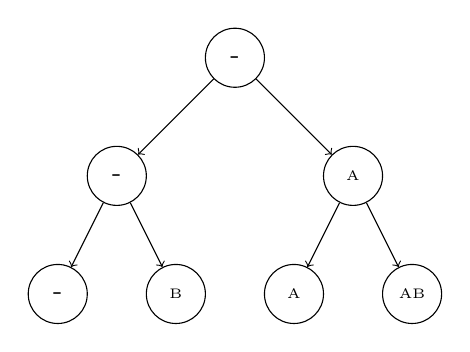
\begin{tikzpicture}[every node/.style={draw,circle, minimum size=0.75cm}, scale=0.75]
	\node at (3, 4) (R) 	{-};
	\node at (5, 2) (RA)	{\tiny A};
	\node at (1, 2) (RO)	{-};
	\node at (6, 0) (RAB)	{\tiny AB};
	\node at (4, 0) (RAO)	{\tiny A};
	\node at (2, 0) (ROB)	{\tiny B};
	\node at (0, 0) (ROO)	{-};

	\draw [->] (R) edge (RA) (R) edge (RO);
	\draw [->] (RA) edge (RAO) (RA) edge (RAB);
	\draw [->] (RO) edge (ROO) (RO) edge (ROB);
\end{tikzpicture}}
    \vspace{2em}
    \sidesubfloat[]{\begin{tikzpicture}[scale=0.75]
	\graph [nodes={draw, circle}, no placement] {
		F[x=3, y=0] -> {R[x=0, y=2], E[x=6, y=2]};
		Z[x=5, y=4] -> {A[x=3,y=4], B[x=4, y=2]};
		A -> {C[x=3, y=6] -> {D[x=0, y=4], R}};
		B -> {E,I[x=2, y=2] -> {R}};	
	};
\end{tikzpicture}}
  \end{center}
  \caption{Beispielgraph und binärer Baum}
  \label{abb:vereinigung}
\end{wrapfigure}
Allerdings gibt es darüber hinaus noch weitere gültige Käufe/Teilmengen. Denn logischerweise können in einer Transakation beliebig viele Firmen des Konglomerates erworben werden. Daher stellt zum Beispiel auch die Menge bestehend aus den Knoten \((A, B) \in V\) und den Knoten, zu denen ein gerichteter Pfad von \(A\) oder \(B\) existiert, eine gültige Transaktion im Sinne der Aufgabenstellung dar.
Denn, um wieder in den Kontext der Aufgabenstellung zurückzukehren, kann der Käufer eine beliebige Firma des Konglomerates entweder unbedingt haben wollen oder den Kauf einer Firma für optional halten. 
Verallgemeinert betrachtet lässt sich eine beliebige Transaktion im Firmenkonglomerat daher als Pfad in einem Binärbaum darstellen. (siehe Abbildung \ref{abb:vereinigung})
Dieser Binärbaum hat als Wurzel die leere Menge. In jeder Ebene n des Baumes stellen die Verzweigungen den Kauf oder das Auslassen des Kaufes von n dar. Somit enthalten die Blätter des Baumes jeden möglichen Kaufwunsch. Ein vollständiger binärer Baum hat \(2^{h-1}\) Blätter \footnote{s. Wikipedia: \url{https://is.gd/cmZlNm}}. Da sich die Höhe des Baumes aus \(V\) und der Wurzel zusammensetzt, folgt daraus, dass es \(2^V\) gültige mögliche "`Kaufwünsche"' gibt.
Die Bestimmung der aufgrund von Nebenbedingungen mitzukaufenden Firmen für \(2^V\) mögliche Kaufwünsche wird bei großer Firmenanzahl sehr zeitaufwändig, schließlich wächst die Blätteranzahl exponentiell zu der Firmenzahl. Allerdings lassen sich diese Mengen auch durch Vereinigungen der Mengen aus dem ersten Berechnungsschritt ermitteln.
Wenn Beispielsweise zum Kauf von \(A\) der Erwerb von \(M_A=\{A, C, D, R\}\) und zum Kauf von \(B\) der Erwerb von \(M_B = \{B, I, E, R\}\) erforderlich ist, ist für den Kauf von \(A\) und \(B\) der Erwerb der Menge \(M_A \cup M_B = \{A, B, C, D, E, I, R\}\) erforderlich (siehe Abbildung \ref{abb:vereinigung}).
Durch die Ausnutzung dieser Eigenschaft lassen sich die Nebenbedingungen der \(2^V\) Kaufwünsche wesentlich schneller bestimmen, denn es können ansatt einer Berechnung im Graphen einfach alle Nebenbedingugngsmengen der ausgewählten Kaufwünsche vereinigt werden.
Eine Betrachtung des eigentlichen Graphens, die per se deutlich komplexer als  die Kombination linearer Mengen sind, wird dadurch vermieden.
Das Blatt, dass unter Einbeziehung der Nebenbedingungen das höchste Gewicht hat, entspricht der gesuchten Teilmenge des Graphens mit dem höchsten Wert.

Die Höhe des binären Baumes lässt sich dank folgender Beobachtung erheblich reduzieren:
Knoten mit einem negativen Gewicht ergeben höchstens als Nebenbedingung Sinn. Es ist sinvoll, eine profitable Firma mit einer unprofitablen Firma als Nebenbedingung zu kaufen, wenn der Gewinn der profitablen Firma den Verlust der unprofitablen Firma übersteigt. Auch ist es sinvoll, mehrere profitable Firmen zu erwerben, deren summierter Gewinn den Verlust einer gemeinsamen unprofitablen Nebenbedingung übersteigt. Firmen mit einem Gewinn von Null ergeben ebenfalls keinen ökonomischen Mehrwert, daher kann auf sie bei der Auswahl der zu kaufenden Firmen verzichtet werden.
Niemals ist es sinnvoll, eine unprofitable Firma direkt zu kaufen. Alle etwaigen profitablen Nebenbedingungen lassen sich auch einzeln kaufen. Daraus folgt, dass der optimale Kaufwunsch nur Firmen mit einem positiven Gewicht beeinhaltet. Daher kann man den Binärbaum auch nur aus den Firmen mit postivem Gewicht aufbauen. Damit sinkt die Anzahl der auszurechnenden Blätter auf \(2^p\), wobei p der Anzahl der Knoten mit positivem Gewicht entspricht.

Die Höhe des Baumes kann noch weiter verkleinert werden. Denn es gibt keinen Grund, eine positivwertige Firma nicht zu kaufen, die nur positivwertige Firmen als Nebenbedingung hat. Bei solchen Teilmengen entsteht ausschließlich Gewinn. Daher können alle Nebenbedingungsmengen aus ausschließlich positivwertigen Firmen zu einer "`Win-Win-Menge"' vereinigt werden. Diese Menge bildet nun die Wurzel des binären Baumes, da sie ja im besten Kauf enthalten sein muss. Die Anzahl der zu berücksichtigenden Blätter ist nun auf \(2^{pm}\) reduziert. \(pm\) entspricht den positivwertigen Firmen, die negativwertige Nebenbedingungen haben.

\section{Heuristik}
Obwohl die Höhe des Baumes nun wesentlich verkleinert wurde, ist amit jedoch nicht das Grundproblem des exponentiellen Wachstums beseitigt. Je nach verfügbarem Arbeitspeicher wird die Zustandsmenge bei einem hinreichend großem \(pm\) irgendwann so groß, dass keine weiteren Zustände mehr gespeichert werden könnnen. Auch ist die Rechenzeit bei einem sehr großen Baum extrem lang. Bei einem Konglomerat mit 169 Firmen (Quadrat-13) müssten ohne Optimierungen beispielsweise \(2^{169}=7,48\mathrm{e}{50}\) Blätter errechnet werden. Dies ist auf einem heutigen Rechner nicht in akzeptabler Zeit möglich.

Für diesen Fall muss dem Algorithmus ein heuristisches Element hinzugefügt werden. Sobald dieses eingesetzt wird, wird nicht mehr mit absoluter Sicherheit die beste Teilmenge gefunden, da Zwischenergebnisse, von denen nicht erwartet wird, dass sie Teil der besten Teilmenge sind, zur Einsparung von Speicherplatz und Verkürzung der Rechenzeit verworfen werden.
In meinem Algorithmus wird, sobald die Zahl der aufgestellten Knoten ein Maximum erreicht, ein Teil der aufgestellten Knoten, also Kaufwünschen, gelöscht. Maximum und prozentualer Anteil der zu löschenden Knoten werdem hierbei zur Laufzeit durch den Nutzer, je nach Genauigkeitsanforderung und zur Verfügung stehender Rechenzeit, festgelegt. Welche Knoten gelöscht werden, entscheidet der Algorithus nach dem Wert des Knotens. Denn es ist deutlich wahrscheinlicher, dass ein Knoten mit hohem Wert ein Zwischenergebniss zum Blatt mit dem höchsten Wert ist, als dass ein Knoten mit vergleichsweise geringem Wert ein solches Zwischenergebniss darstellt. Während der Entwicklung hat sich ein Maximum 50'000 Knoten und eine Löschquote von 50\% als ein geeigneter Kompromiss aus Laufzeit und Genauigkeit herausgestellt.

Für meinen Algorithmus lautet die Antwort auf Teilaufgabe 3 "`it depends"'. Solange die Knotenzahl das vom Nutzer gesetzte Maximum unterschreitet, findet das Programm mit absoluter Sicherheit die beste Teilmenge, schließlich wird der gesamte Entscheidungsbaum aufgebaut. Sobald das Maximum überschritten wird, ist nicht mehr sicher, dass das beste Ergebnis gefunden wird. Schließlich wurde der Baum nicht komplett aufgestellt. Die Wahrscheinlichkeit, dass trotzdem das korrekte Ergebnis gefunden wird, kann der Nutzer dadurch erhöhen, dass er das Programm anweist, weniger Zwischenergebnisse zu verwerfen.